\documentclass[fleqn,s1,tex]{neptune}
\usepackage[5.5]{neptune-els-dtd}
%% Please do not edit bookindate/proofdate
\bookindate{2019-05-10}
\proofdate{2019-05-15}
%%
\usepackage[nptn]{neptune-els}
\usepackage{graphicx}
%\usepackage{subcaption} 

\begin{pkg}
\end{pkg}

\begin{additionalpkgs}
\end{additionalpkgs}

\begin{document}

\newproof{proof}{Proof}

\begin{macros}

 \newcommand*\rot{\rotatebox{90}}
\end{macros}

\begin{additionalmacros}
\def\rvtLingua{Lingua}
\jshort
\end{additionalmacros}

\begin{frontmatter}
%\QUERY[1]

\title{Language features in extractive summarization: \\Humans Vs. Machines}
\tnote{\cfino}

\addrai[1]{S0950705119302205-93af51ede5bb70b7edcb1f03155c6cb1} 
 \addrai[2]{S0950705119302205-8ce426376d9335de21afeef2abd9a36a} 
 \addrai[3]{S0950705119302205-b45266e06a959017fa3b57c0443aa7c2}



\begin{authorgroup}

\author[mymainaddress]{Ignacio Arroyo-Fern\'andez}
%\QUERY[2]
\cormark[1]
\cortext[1]{\COR
}
\email[iaf@ccg.unam.mx]

\author[mysecondaryaddress]{Arturo Curiel}
\email[acuriel@conacyt.mx]

\author[mythirdaddress]{Carlos-Francisco M\'endez-Cruz}
\email[cmendezc@ccg.unam.mx]

\affiliation[mymainaddress]{o={Universidad Nacional Aut\'onoma de M\'exico (UNAM), Ciudad Universitaria, CDMX}, cy={Mexico}}

\affiliation[mysecondaryaddress]{o={CONACYT - Universidad Veracruzana - Facultad de Estad\'\i stica e Inform\'atica},
a={Av. Xalapa Esq. Manuel \'Avila Camacho s/n, 91020, Xalapa}, c={Veracruz}, cy={Mexico}} 

\affiliation[mythirdaddress]{o={Centro de Ciencias Gen\'omicas, Universidad Nacional Aut\'onoma de M\'exico, Av. Universidad},
a={s/n, Colonia Chamilpa, Cuernavaca-Morelos 62100}, cy={Mexico}}
\end{authorgroup}

\begin{abstractgroup}
\begin{abstract}[1]
This paper presents a comparative statistical analysis of the language features most commonly used for Automatic Text Summarization (ATS), namely: Parts of Speech (PoS) (unigrams and bigrams), sentiments (by token and sentence), and Rhetorical Structure Theory (RTS) relations. The analyses were carried out on both human-made and machine-made summaries, in order to determine whether current ATS systems capture the same kind of information as humans do. 
 Our results show that there are some marked differences between machine and human-made summaries, which at times may seem counterintuitive. For instance, named entities were usually frequent in machine-made summaries, but not in human-made ones. Similarly, words perceived to hold a ``neutral'' sentiment were systematically favored by machines, but not always by humans. 
\end{abstract}
\begin{abstract}[7]%\QUERY[3]
\begin{itemize}
\item This paper investigates pertinence of language features commonly utilized in ATS. 
\item Statistical comparisons were conducted between human-made and machine-made summaries.
\item Some features were interestingly used moderately by humans, but not by machines.
\end{itemize} 
\end{abstract}
\keywords{Automatic text summarization \sep Statistical feature analysis \sep Natural language processing \sep Artificial intelligence}
\end{abstractgroup}


\end{frontmatter}

\section{Introduction}

\xlabel{intro}

\textit{Automatic Text Summarization} (ATS) is the Natural Language Processing (NLP) task that deals with the creation of condensed versions of either one or multiple documents (\textit{sources} or \textit{source documents}) by extracting their most relevant information~\cite{radev2002introduction}. A system that performs the ATS task is usually called a \textit{summarizer}. 

There are two main types of ATS: \textit{extractive summarization} and \textit{abstractive summarization}. An extractive summarizer creates summaries by selecting sentences from the source documents that it deems \textit{relevant}; the selected sentences are added, without modification, to the final result. Conversely, an abstractive summarizer reworks the sources' relevant information into an intermediate meaning representation layer, where it is possible to use techniques from Natural Language Generation (NLG) to generate a summary from scratch.

Extractive rather than abstractive summarization has traditionally been the most favored ATS solution throughout the years. Multiple extractive ATS methods exist, whereas few abstractive ones are available. The most common approaches are based on topic segmentation, graph representation, discourse labeling and, in general,
Machine Learning (ML) techniques~\cite{gambhir2017recent}. 

Regardless of the technique, every summarizer has to deal with the issue of how to automatically quantify the relevance of the source information, which for humans may depend on subjective
criteria~\cite{barry_user-defined_1994,barry_users_1998,taylor_user_2012}. Furthermore, even if a good measure of relevance can be found, there is no a reliable definition of what a good summary is. Thus, existing ATS efforts only look at how to maximize the information content from the sources in the summaries, which may not always be the goal of a human summarizer~\cite{nandhini_improving_2013}. 



Several well-known statistical ATS evaluation methods consider lexical
overlapping as an indicator of how good a summary is. The standard approach uses the Recall-Oriented Understudy for Gisting Evaluation (ROUGE) metric. This metric is considered sufficiently accurate and is based on measuring the overlap of lexical items between human-made and machine-made summaries~\cite{conroy2008mind,lin:2004rpa}.  Thus, existing automatic summarizers try to maximize the overlap of the most significant terms as measured by ROUGE~\cite{galanis2012extractive}. This paper conveniently adopts the point of view of Artificial Intelligence, from which it is desirable that machine-made summaries be as similar as possible to human-made ones. In this sense, scores based on lexical overlap are probably not sufficient to fully assess this similarity.



As pointed out by~\cite{kdir16}, there is an imbalanced use of lexical features by automatic summarizers, which contrasts with humans performing the same task. Indeed, some language features like named entities, verb--noun bigrams and prepositions are usually overrepresented. Only recently have other alternative features like word and sentence sentiments been used for extractive
summarization~\cite{BHARGAVA2016404}, but they remain unexplored formally as features. 

In this work, the basics of the ATS task are revisited by contrasting the statistical differences between machine-made and human-made summaries in the sense of language usage. This is an attempt to identify commonly overlooked features in ATS, which can provide cues of relevance independently of the lexical overlap between sources and their corresponding summaries.
  
Our analysis was performed over three different groups of summaries: human-made, state-of-the-art and baseline machine-made summaries. The summaries were created from sources in three different domains: news articles, movie synopses and scientific abstracts~\cite{hong2014improving}.

In general, the analysis of the summaries was divided in two stages. In both stages, three kinds of feature were considered: Parts of Speech (PoS), sentiments (at token and sentence levels) and Rhetorical Structure Theory (RST) tags. In the first stage, all features were analyzed from the point of view of the three groups of summaries. This consisted in computing the \textit{Feature Spectrum} of a set of features, which is a statistical measure of the $\log$ differences between feature counts of human-made summaries and feature counts of machine-made summaries~\cite{kdir16}. In the second stage, each feature was analyzed individually for the three summary groups. A whisker diagram (boxplot) was plotted for each feature and for each summarizer (either human or machine), showing the similarities/differences between the quartiles of the groups of summaries. The hypotheses suggested by such similarities/differences were also supported/rejected by using a well-known nonparametric statistical test for small non-Gaussian-distributed sample sizes, i.e.~the Mann--Whitney U test~\cite{SMALHEISER2017157}. In addition, a linguistic point of view of the described behavior was provided when applicable.

The results showed marked differences between human-made and machine-made summaries, particularly regarding the use of features such as dates, bigrams of proper nouns and sentiments per-word and per-sentence. Importantly, these differences could also be observed in summaries done by state-of-the-art systems. 

To the best of the authors' knowledge, this is the first study to directly compare humans against machines in the sense of features for the ATS task, and it could be useful to improve future ATS efforts by highlighting language features that are currently ignored by machines, but not by humans. In turn, this could also point towards novel summary and NLG evaluation techniques that may take into account these newly reported features.

The rest of this article is organized as follows. \xref{sec02:methodology} presents the methodology employed to perform the experiments, the features that were studied and the experiment setup. \xref{sec03:dataAndTools} provides a description of the datasets and software tools. \xref{sec04:resultsAndDiscussion} presents both the obtained results and their discussion. Finally, \xref{sec05:conclusions} presents the conclusions.

 \section{Methodology}
 \xlabel{sec02:methodology}
We performed the statistical comparison of several features extracted automatically by means of state-of-the-art implementation of PoS, RST and sentiment taggers from all the summaries contained in publicly available datasets (\xref{sec:humanDatasets,sec:machineDatasets}). To begin our comparison, we reviewed some features widely used in previous works to assess how relevant they actually are to characterize the summaries as generated by humans or by machines. This defined a general set of features selected from the whole set extracted by means of well-known tagging tools. From this set of features and from the first part of our analysis, we selected another subset of them, which we considered to be \textit{pertinent}.

\begin{figure}%1
\caption{The general block diagram of our methodology\xlabel{fig:block_diagram}}
\includegraphics{Figure_1}
\end{figure}

Regarding the machine-made summaries we analyzed, they are $100-$word
 news documents generated by automatic summarizers contained in an inventory built by~\cite{hong2014repository}, which includes two categories of summarizers: state-of-the-art and baseline. The categorization was performed by the authors of the inventory according to different versions of the ROUGE measure that the summaries obtained on the corresponding DUC-2004 task (\xref{sec:machineDatasets}). We adopted such categorization as two different groups of summaries to compare against humans, the third group. 

Regarding the human-made summaries, part of them were $100-$word news documents taken from the DUC-2004 dataset (\xref{sec:humanDatasets}). The groups of human-made summaries was also enriched with movie synopses and scientific paper abstracts (see Section \xref{sec03:dataAndTools}). It helped us to select features that were, as much as possible, not dependent on the domain of the texts and on the summarizers. 

Our statistical comparison was two-fold (see \xref{fig:block_diagram}). The first part of our analysis consisted in using the method called \textit{Feature Spectrum} to compare the three groups of summaries. This method has been extensively used in engineering before; for instance, to compare sound power levels with respect to a reference level. This method does not provide information about individual annotators/summarizers. Thus, the resulting comparison showed us a general portrait of how the frequency of occurrence of each item of the general set of features helped us to observe how much humans and machines differed~\cite{kdir16}. To compute the Feature Spectrum we used a \textit{fitting dataset}, including the three groups of summaries generated by humans and machines randomly drew from the whole dataset of summaries.\footnote{In this work we prefer the term ``fitting dataset'' instead of the term ``training dataset'' which is commonly used among the members of the Machine Learning community. However, note that in this paper we are not training any specific model.}

Given a language feature $f_i$, e.g.~bigrams of nouns, we computed its frequency within each item of a set of human-made summaries, $H$ (the reference group), and a set of machine-made summaries, $M$ (the under-study group). Thus, for human-made summaries, we represented the feature as the median $\varphi_H(f_i)$ of the frequencies of $f_i$ within $H$. For machine-made summaries the median frequency for the same feature is denoted by $\varphi_M(f_i)$. We use the ratio in \xref{eq:spectrum}, or \textit{log} difference, as an item of the Feature Spectrum $\mathcal{F}\ni F_i$ to compare groups of  machines and also to compare them with humans, and with respect to $f_i$: 
\begin{equation}
\xlabel{eq:spectrum}
F_i=20\log \frac{1+\varphi_M(f_i)}{1+\varphi_H(f_i)}.
\end{equation}
See the definition and interpretations of $\mathcal{F}$ in Section 3 of Supplementary material (\xref{sec:appendix}).
%\footnote{\myehost{https://github.com/iarroyof/summ_features/blob/master/KNOSYS-D-18-02363R1_supplementary.pdf}.} 

 During the second part of our analysis, we compared all sampled summaries (human- and machine-made) focusing on the pertinent set of features coming from the Feature Spectrum analysis performed on the fitting dataset. Such features showed a tendency to help to distinguish two or three of the groups of summaries. This was assessed by comparing boxplots derived from the same fitting dataset, which provided a number of hypotheses of the form: 
\begin{itemize}         
     \item $H_0: $ ``The distributions of the feature $f_i$ in the groups of summaries $H$ and $M$ are statistically \textit{independent}''.
     \item $H_1: $ ``The distributions of the feature $f_i$ in the groups of summaries $H$ and $M$ are statistically \textit{dependent}''.
\end{itemize}

Next, we built a \textit{development dataset} of random samples for each of the pertinent features. It is important to note that the summaries it contained were not present in the fitting dataset, and were also grouped in two groups of machine-made summaries and one group of human-made ones. Afterwards, we computed Mann--Whitney U tests on the development data in order to assess what hypotheses were/were not worth supporting~\cite{du2009confidence}, e.g.~``The group of summaries $H$ is statistically dependent of the group $M$'' with probability $P<0.05$, were $P<0.05$ also reads ``the $p-$value is less than $0.05$''. In the case of this particular example, $0.05$ is the upper limit to consider that the null hypothesis $H_0$ is worth supporting: statistical independence. Otherwise, $P\geq 0.05$, the alternative hypothesis $H_1$ (statistical dependency) is considered as worthy of acceptance. The obtained $p$-values also supported the reproducibility of our results, and we summarized several of them using heatmaps that represented the probabilities $P$ as color intensities. The Mann--Whitney U test is nonparametric, and it has been considered as the workhorse for comparing unpaired non-Gaussian-distributed samples of small sizes~\cite{SMALHEISER2017157}.

\subsection{Analyzed Features}

The hypothesis behind our study is that relevance is not only encoded in lexical items of text, but also in the structure of
language~\cite{harris1957co,Harris1991information,jones1999automatic}. As a first approach to confirm the hypothesis, we investigated whether language features other than lexical items are so relevant for a summary in such a way that simply their frequencies of occurrence can be used to characterize it well. These features are used by a number of extractive summarizers to detect relevant fragments of the source document. Nonetheless, in most cases the features are either used independently by different summarizers or used for adding information to summarizers so as to maximize evaluation scores~\cite{hong2014improving}. 

PoS tags are among the most popular features in the literature, also they are the most related to structure of language. Thus, our hypothesis can benefit from taking them into account when computing feature statistics.  Other popular features are named entities (NEs). The intuition behind such features (proper nouns, dates, quantities, etc.) is that when a document mentions an entity, it is possible that relevant information is anchored to it. This relevance is mainly associated to the particular domain of the source document. In this
sense, NEs are by themselves relevant. Another interesting feature is sentiment polarity, and it has been used
recently in ATS~\cite{BHARGAVA2016404,dabholkar2016automatic,yadav2016text}. We extracted from summaries the sentiment polarities of words and sentences with the following tags: \textit{very negative, negative, neutral, positive} and \textit{very positive}. 

We compared an additional kind of language feature that has been used few times in ATS literature. It characterizes language structure at the discourse level. The idea is to take into consideration different levels of language beyond lexical items and syntax, then, studying discourse structure in summaries could be relevant. The Rhetorical Structure Theory (RST) establishes discourse relations among fragments of text called elementary discourse units (EDUs). We tagged these relations and tried to characterize summaries based on discursive
attention~\cite{grosz1986attention}. Some examples of these relations are: \textit{Background, Circumstance, Concession, Condition, Purpose, Cause and Result}~\cite{mann1988rhetorical}. 

\section{Data and Tools}
\xlabel{sec03:dataAndTools}
\subsection{Human-made summaries}
\xlabel{sec:humanDatasets}

In this work, we use popular datasets in the ATS literature. This is the case of the DUC-2004 dataset, which contains short human-made summaries and the source documents they were generated from. In addition, we included movie synopses and abstracts of scientific papers, which we consider to be linguistic samples intentionally written to summarize information. 

\paragraph*{The \?{DUC}-2004 dataset}

The DUC-2004 is a multi-document summarization dataset which is constituted by 50 clusters (topics/timestamps) of text documents.\footnote{\myehost{http://www-nlpir.nist.gov/projects/duc/data/2004_data.html}.} Each of them comes from $10$ source documents that are journalistic notes.

We used only the human-made summaries from this dataset. Eight different annotators (human summarizers) provided the summaries. Each annotator generated $25$ $100-$word summaries. This number of summaries per annotator (both for humans and machines) is the minimum assigned to the groups we studied in this work.

\paragraph*{The movie synopsis dataset}

The movie synopsis dataset\footnote{\myehost{http://www.cs.cmu.edu/~ark/personas/}.} was extracted from Wikipedia (2012). The authors of this dataset selected synopses containing essential actions and character traits characterizing a particular movie. This selection produced $42306$ summaries in total. The summaries contain $176$ words on average. To build our fitting and development data we randomly selected only those that contained between $100$ and $120$ words in order to correspond to the number of samples available per annotator in the DUC-2004 dataset. The movie synopses have no metadata identifying the annotator. In this way, this dataset helped us to assess our language feature analysis independently of the specific individuals wrote the synopses.

\paragraph*{The \?{NIPS} papers dataset}

This dataset consists of abstracts of scientific papers from the Neural Information Processing Systems (NIPS) conference. The papers are those published from the first conference held in 2007 up to a recent conference held in 2016.\footnote{\myehost{https://www.kaggle.com/benhamner/nips-papers}.} We selected only those abstracts that contained between $100$ and $120$ words. We also drew a random sample while keeping $25$ summaries per annotator. Although in this case authorship metadata was available, we ignored it in order to keep the experiments independent of annotators, as in the case of the movie synopses dataset.

\subsection{Machine-made summaries}
\xlabel{sec:machineDatasets}

\paragraph*{The \?{S}um\?{R}epo dataset}

The SumRepo dataset is composed of $600$ documents which were obtained from the Task-2 of the DUC-2004 benchmark. These documents are machine-made \ubrk summaries and correspond to the output of both state-of-the-art and baseline systems categorized by using different ROUGE scores. The summaries were generated by $12$ systems in total (see a description of selected summarizers, their evaluation scores and their categorization, Tables 2 and 1, in Section 1 of Supplementary material), and each system generated $50$ summaries in turn. Each summary was generated from a whole cluster of source documents dealing with a topic in the DUC-2004 dataset (\xref{sec:humanDatasets}). In order to keep the limit of $25$ summaries per annotator, we randomly selected $25$ summaries from $50$ summaries generated by each system. This gave us $200$ documents of $\sim 100$ words each ($665$ bytes). The lower scores are provided by baseline systems and the higher scores by state-of-the-art systems. See Tables 1 and 2 in Supplementary materials.

For human-made and for machine-made summaries we drew two random datasets with equal characteristics but from different source documents. These two datasets were named fitting data and development data, respectively.

\subsection{Tools}


It was relevant to our study that features were
tagged automatically in order to make it practical, reproducible and unbiased from human judgment. Part-of-speech tagging as well as sentiment tagging were performed using the Stanford
CoreNLP~\cite{manning2014corenlp}.\footnote{\myehost{https://stanfordnlp.github.io/CoreNLP/}.}
This is a state-of-the-art system for natural language processing with several annotation tools. The sentiment features we analyzed were identified by the sentiment classifier included in CoreNLP. It takes into account structural features by propagating the learning error from top to bottom through a
(recursive) tree~\cite{socher2013recursive}. The classifier estimates sentiments for phrases based on their constituent words embedded into its parameter space. The classes are sentiments polarities known in advance: \textit{very negative, negative, neutral, positive} and \textit{very positive}.

RST relations (EDUs) were tagged using the implementation and directions detailed in~\cite{feng2014linear}. It is a parser that produces discourse tree structures from raw text. 

 To count feature frequencies, compute Feature Spectrum, generate boxplots and
plot heatmaps of $p$-values we used the statistical analysis and visualization tools
provided by~\cite{deardorff2016tableau,mckinney-proc-scipy-2010,Hunter:2007}.

\section{Results and Discussion}
\xlabel{sec04:resultsAndDiscussion}

\subsection{The Feature Spectrum}

 We computed the Feature Spectrum defined in \xref{sec02:methodology} as a general approach to compare feature usage between human and machine made summaries. In \xref{fig:spectrum}, the feature names $f_i$ are on the horizontal axis and their corresponding (signed) levels $F_i\in\mathcal{F}$ are on the vertical axis. According to the Feature Spectrum, if we have, for instance, $F_i=6$ (positive) in baseline summaries, it means that $f_i$ usage in these summaries is double that of the human-made summaries (i.e.~an excess of $10^{\frac{6}{20}}\approx 2$). Otherwise, if we have $F_i=-6$ (negative), it means that $f_i$ feature usage in baseline summaries is half as frequent in human-made summaries in comparison with machine-made summaries (i.e.~a lack of $10^{\frac{-6}{20}}\approx 1/2$). See Section 3 of Supplementary material for details. The Feature Spectrum assumes human levels as references, so $F_i=0.0$ for all $f_i$ in human-made summaries. Machine-made summaries around this level are considered of equal or very similar behavior with respect to human-made ones.

\begin{figure}%2
\caption{The Feature spectrum is  used to identify a set of pertinent features\xlabel{fig:spectrum}}
\includegraphics{Figure_2}
\end{figure}


We observed that there were some features whose usage levels in machines (baseline and state-of-the-art) was very similar to what was observed in humans (\xref{fig:spectrum}). This is the case of \texttt{sent\_sentim\_1}, \texttt{sent\_sentim\_2}, \texttt{NNS\_MED}, \texttt{NNS\_PERIOD}, \texttt{NNPS\_AVG}, \texttt{NNPS}, \texttt{CD\_MAX} and \texttt{CD\_MED} (see the description of these features in Supplementary Table 3). Notice that they can also be interpreted as uninformative in distinguishing either humans from machines or machines from other machines. 
%\QUERY[4]
\begin{figure*}%3
\caption{Boxplot of the date (\texttt{DATE}) feature through all summaries. Horizontal axis indicates the human/machine summary. Vertical axis indicates the frequency of occurrence of the feature\xlabel{fig:DATE}}
\includegraphics[scale=0.25]{Figure_3}
\end{figure*}

Other features allowed us to note what all machines did similarly, but differently with respect to humans. For example, the feature \texttt{tok\_sentim\_3} (the amount of tokens with positive sentiment polarity) was found to be half as frequent in machine-made summaries in comparison with human-made ones, i.e.~$10^{\frac{-6}{20}}\approx \frac{1}{2}$. Conversely, the feature \texttt{DATE} (the amount of date mentions) was found to be about $10^{\frac{13}{20}}\approx 4.46$ times more frequent in machine-made summaries than in human-made ones. Therefore, humans maintain an economic use of dates when compressing information, while machines do not have this ability.

The Feature Spectrum also allowed us to distinguish baseline summaries from state-of-the-art ones. This is the case of features \texttt{CC}, \texttt{tok\_sentim\_1}, \texttt{TotalRST}, \texttt{no\_openie}, \texttt{no\_tokens}, \texttt{tok\_sentim\_2}, \texttt{IN}, \texttt{IN\_AVG}, \texttt{IN\_MIN}, \texttt{IN\_NNP}, \texttt{no\_corefs}, \texttt{VBD}, \texttt{VBD\_AVG}, \texttt{NNP}, \texttt{NNP\_MAX}, \texttt{NNP\_AVG}, \texttt{NNP\_MED}, \texttt{NNP\_VBZ}, \texttt{NNP\_NN},  \texttt{NNP\_NNP}, \texttt{named\_entities}, \texttt{NNP\_AVG}, \texttt{NNP\_MIN}, \texttt{NNP\_IN} and \texttt{DATE}. Thus, in most of the pertinent features, human usage cannot be imitated by machines.

Surprisingly, some features indicated that baseline summaries were more akin to humans than state-of-the-art summaries. The most notable instance of this behavior was for the \texttt{NNP\_VBZ} feature. State-of-the-art machines used it excessively by a factor of $10^{\frac{6}{20}}\approx 2$, while baselines kept $F_i\approx 0.0$. A linguistic argumentation for this is that a proper noun followed by a verb refers to a volitional subject doing an action, which could very likely be a relevant part of the discourse. However, humans can decide which of these parts are truly relevant, while machines cannot. Also negative instances were \texttt{tok\_sentim\_1}, \texttt{TotalRST}. In the case of \texttt{CC} (coordinating conjunctions), baseline machines were shown to be nearer to humans ($10^{\frac{-2}{20}}\approx 0.8$) than state-of-the-art machines ($10^{\frac{-4.5}{20}}\approx 0.6$), but groups of machines showed a lack of use of this feature. 

The Feature Spectrum also showed how state-of-the-art summaries were more akin to humans than baseline summaries. The features involved here represent the main differences observed between state-of-the-art and baseline summaries (right hand side of \xref{fig:spectrum}): \texttt{no\_openie}, \texttt{no\_tokens}, \texttt{tok\_sentim\_2}, \texttt{IN},  \texttt{IN\_AVG},  \texttt{IN\_MIN}, \texttt{no\_corefs},  \texttt{NNP\_MAX}, \texttt{VBD\_AVG}, \texttt{NNP\_AVG}, \texttt{NNP\_MED}, \texttt{NNP\_NN}, \texttt{named\_entities}, \texttt{NNP},  \texttt{IN\_NNP}, \texttt{NNP\_NNP}, \texttt{NNP\_MIN}, \texttt{NNP\_IN}, \texttt{VBD} and \texttt{DATE}. Overall, human use of these features was much harder for machines to imitate. The case of \texttt{NNP\_NN} (bigrams formed by a singular proper noun and a singular common noun) is an exception for state-of-the-art machines. Commonly, an \texttt{NNP\_NN} compresses information into two words (i.e.~nominalization).

Sentiment features showed interesting behavior, although, usually, they are not considered language features. For the Feature Spectrum, we considered all sentiment polarities provided by the CoreNLP tool. It is notable that machines showed a meaningful lack of positive sentiments. The case of neutrality of words (\texttt{tok\_sentim\_2}) is no less notable because it was easy for state-of-the-art machines to imitate. Nevertheless, they find it very hard to express positive (\texttt{tok\_sentim\_3}) and negative (\texttt{tok\_sentim\_1}) sentiment polarities.\footnote{It is inevitable that this fact evokes the HAL-9000 computer from the well-known novel and film entitled \textit{``2001: A Space Odyssey''} by Arthur C. Clarke.} 
%\QUERY[5]
\begin{figure}%4
\caption{Mann--Whitney U test for \texttt{DATE} mentions in human-made and machine-made summaries \uscoltext
\xlabel{fig:date_heatmap}}
\includegraphics[width=8.7cm,height=7.5cm]{Figure_4}
\end{figure}

\subsection{Hypothesis tests}

In this section we analyze statistical differences among the groups of summaries we studied, i.e.~human-made summaries and machine-made summaries (the latter group is in turn divided into state-of-the-art and baseline summaries). In order to assess such differences, we performed a fine-grained analysis focused on the frequency of occurrence of a set of features showing interesting behavior during Feature Spectrum and boxplot analysis such that they allowed us to distinguish groups of summaries. 

\begin{figure*}%5
\caption{Boxplot of the proper noun bigrams feature (\texttt{NNP\_NNP}) through all summaries. Horizontal axis indicates the human/machine summary. Vertical axis indicates the frequency of occurrence of the feature\xlabel{fig:NNP_NNP}}
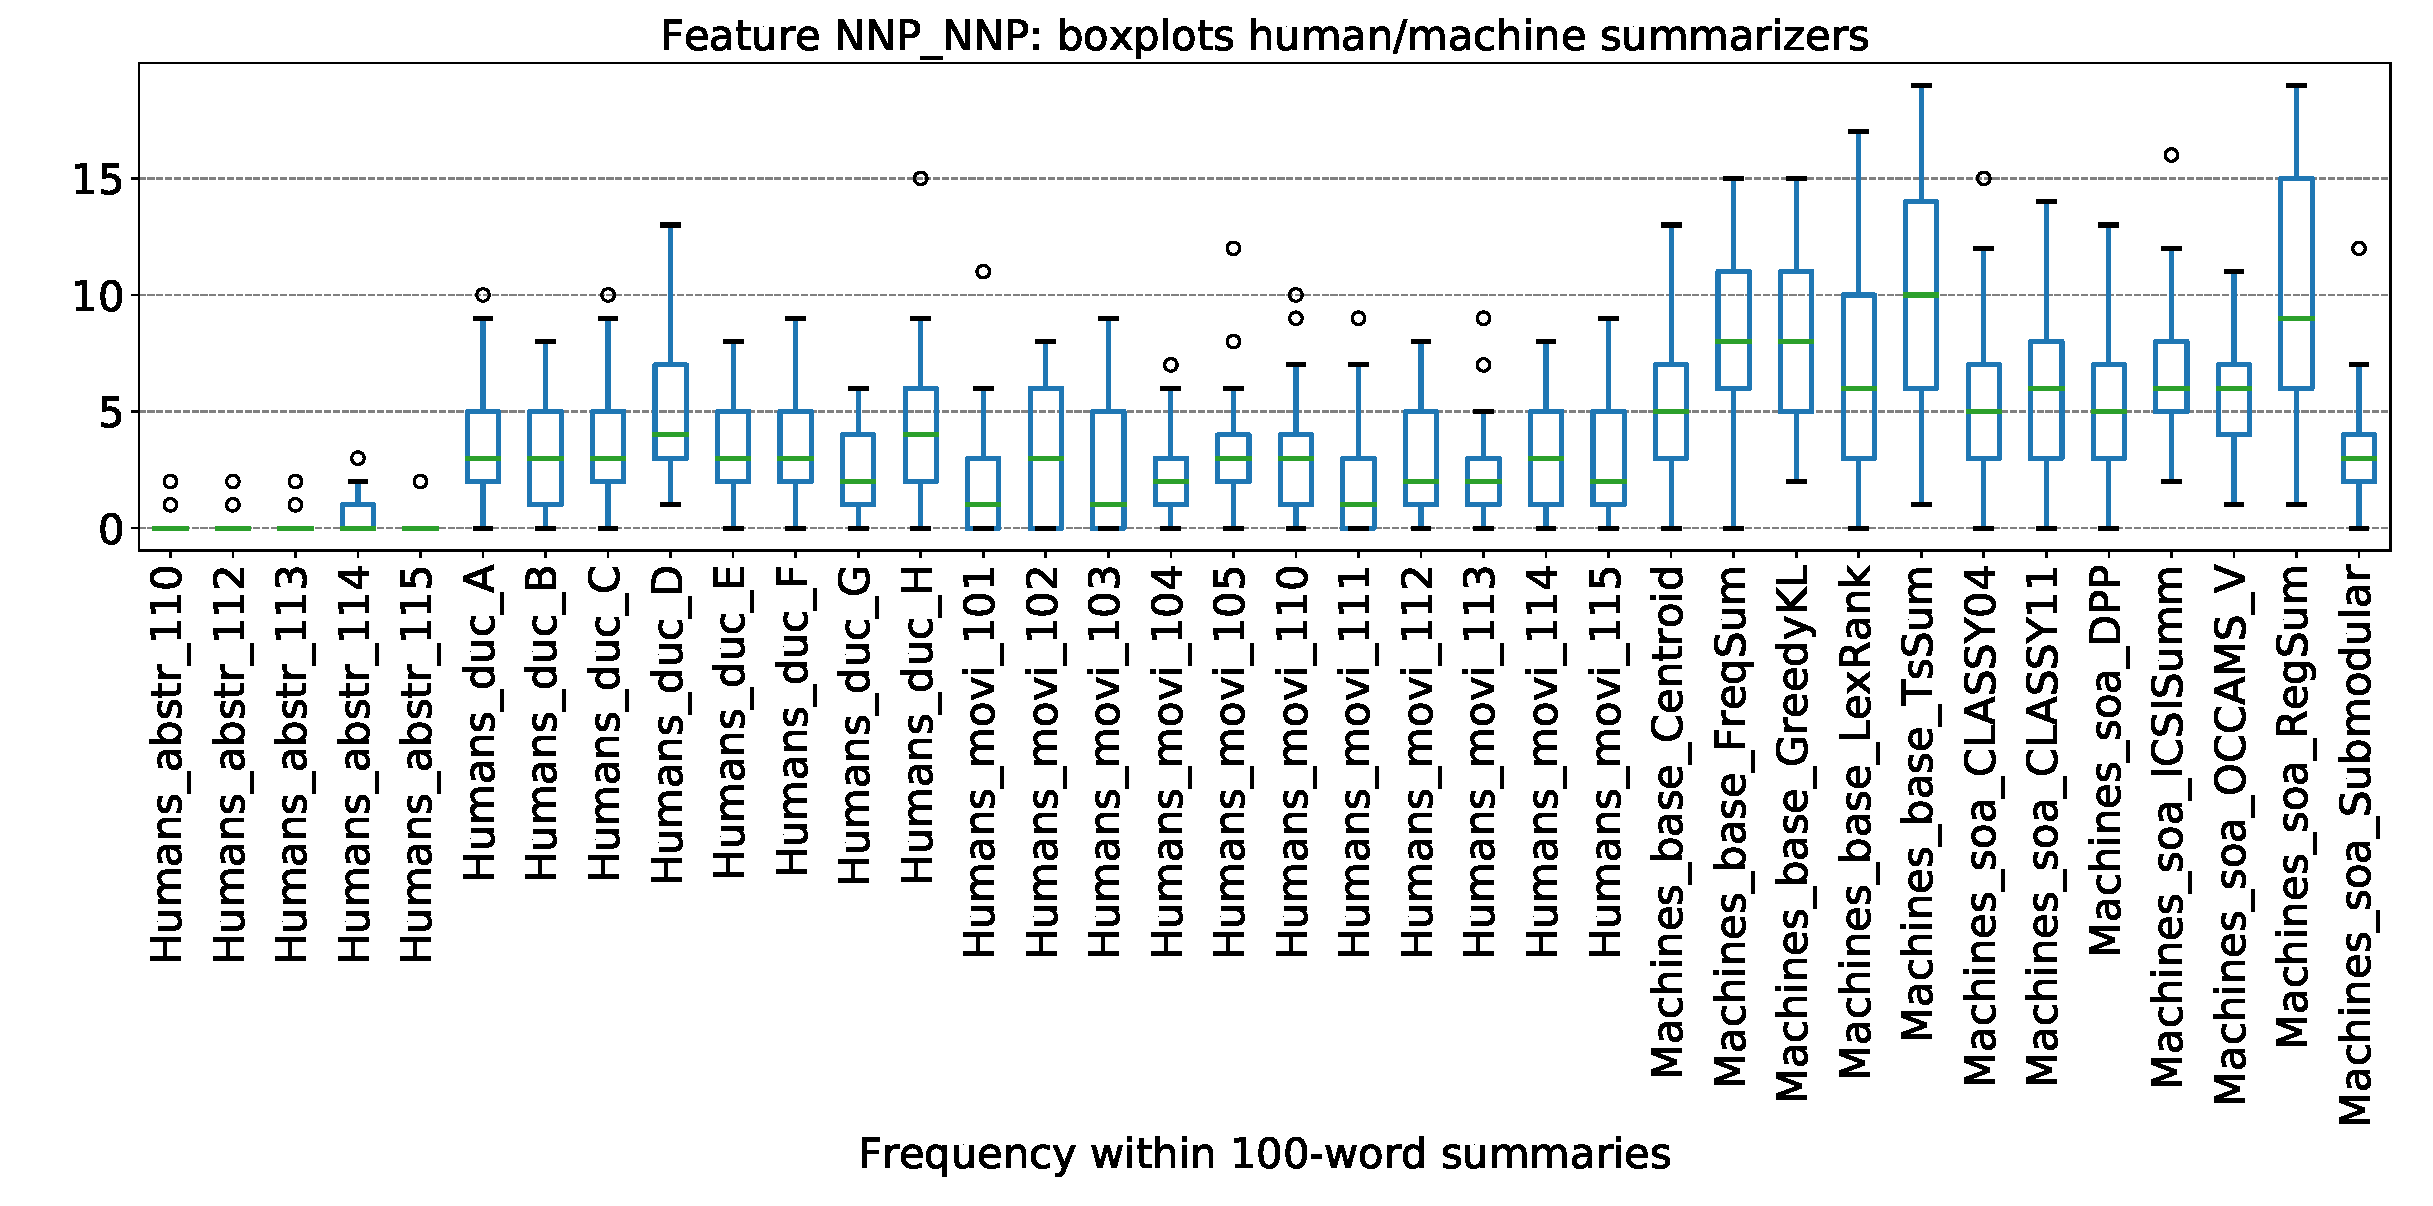
\includegraphics[scale=0.25]{Figure_5}
\end{figure*}
\nosubfloat

\begin{figure*}%6
\caption{Boxplot of (a) the median of proper nouns by sentence (\texttt{NNP\_MED}) and of (b) the frequency of named entities (\texttt{named\_entities}) through all summaries. Horizontal axis indicates the human/machine summary. Vertical axis indicates the frequency of occurrence of the feature.}
\subfigure[]{\xlabel{fig:NNP_MED}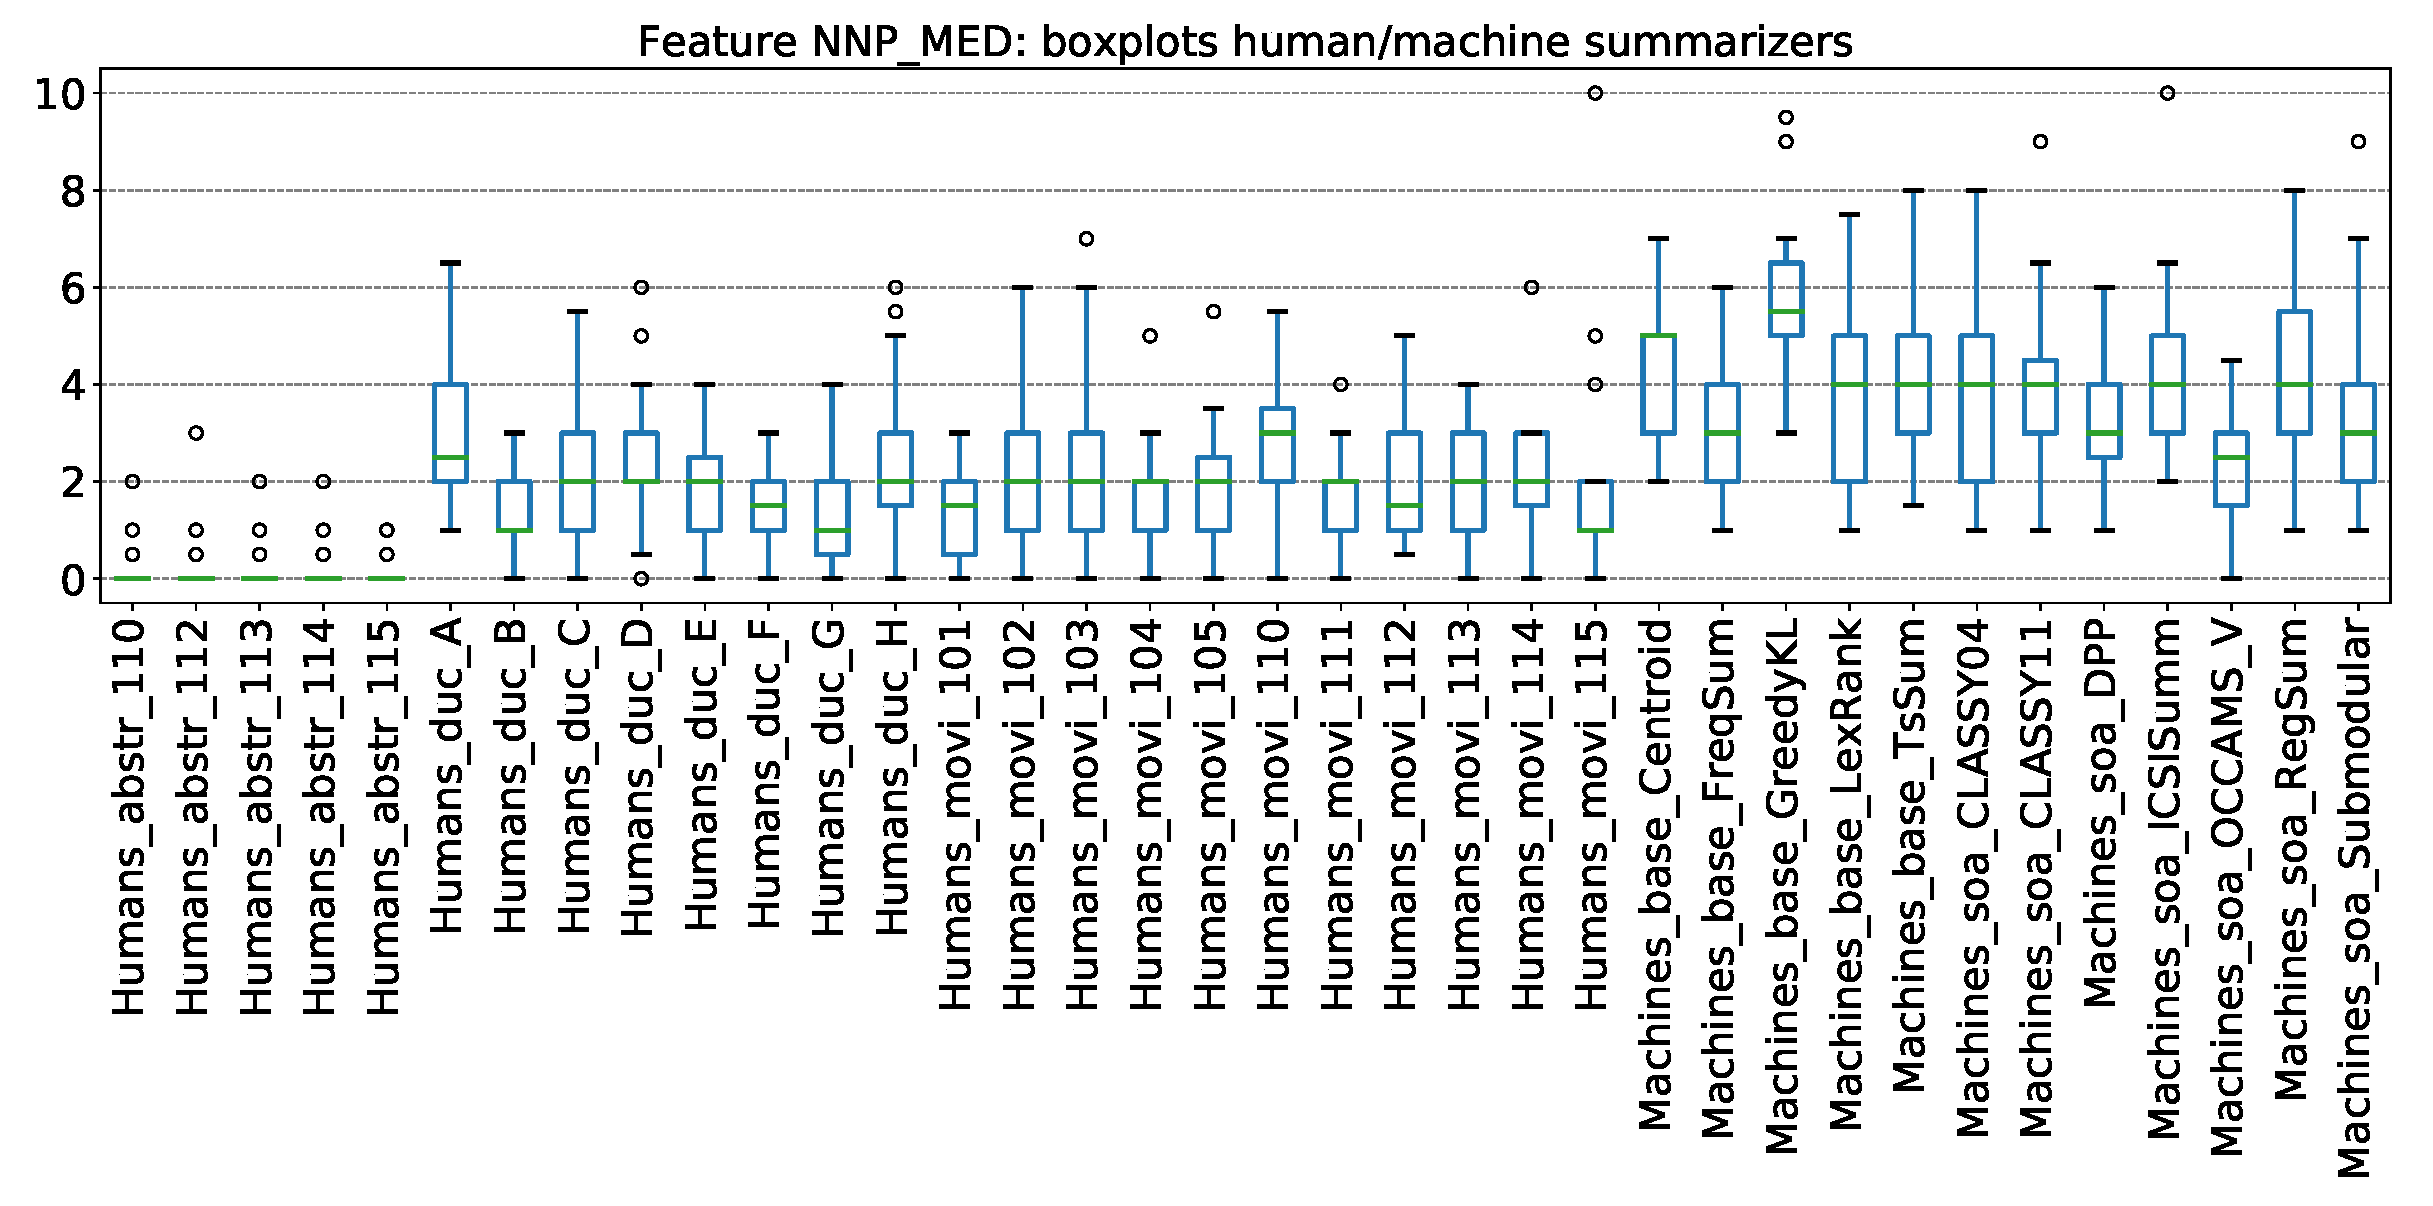
\includegraphics[scale=0.25]{Figure_6a}}
\subfigure[]{\xlabel{fig:named_entities}\includegraphics[scale=0.25]{Figure_6b}}
\end{figure*}

The Feature Spectrum analysis was in turn decomposed into two stages. First, feature frequency statistics were observed using comparing boxplots. For this stage, we used the fitting dataset of summaries, i.e.~the same data used during Feature Spectrum analysis. The second stage of experiments was conducted on a different set of summaries. We refer to this dataset as development data.\footnote{Fitting data, development data and raw $p$-values of our experiments can be found at: \myehost{https://github.com/iarroyof/summ_features/tree/master/heatmaps}.} This was constituted by samples coming from different source documents other than the samples in the fitting dataset. The experiments conducted on the development data aimed to assess statistical significance of Feature Spectrum analysis. 


The criterion for pertinence of a given feature was that it allowed for the three groups of summaries (or two of them at least) to be distinguished. The Feature Spectrum gave a general view of this. Once this general view helped to identify pertinent features we analyzed the summaries produced by each different source (either human or machine) producing the groups of summaries of the given feature by using boxplots. If most samples generated by humans did not overlap within the interquartile range (IQR) of those generated by machines. The same comparison was considered for distinguishing summaries generated by state-of-the-art machines from those generated by baseline machines. In addition to the identification of features relevant to distinguish groups of summaries, this procedure also gave us insight into similar behaviors between humans and machines when creating summaries. 

We selected three features that showed interesting behavior according to the Feature Spectrum. Then, we performed fine-grained analysis using their boxplots: dates (\texttt{DATE}), proper noun bigrams (\texttt{NNP\_NNP}) and neutral sentiments by token \ubrk (\texttt{tok\_sentim\_2}). 


It could be observed that \texttt{DATE} is commonly absent in most human-made summaries (\xref{fig:DATE}). Contrarily, this feature is relatively frequent in machine-made summaries. Particularly, in most cases, the median of the number dates in machine-made summaries did not overlap the IQR of human-made ones (and vice versa). Among the few exceptions of this observation, the most notable was observed for the human-made summaries generated by the annotator identified as \texttt{Humans\_duc\_A} (shown on the right hand side of the figure). This annotator used a median of about $5$ dates (and $15$ dates maximum). This is much more than what was observed for other annotators and other groups of human-made summaries, regardless of whether they are paper abstracts, news or movie synopses. It should also be noted that the median number of dates employed by this annotator surpassed the medians of all machine-made summaries. Furthermore, this median did not overlap the IQR of any other group of human-made summaries, which constitutes atypical behavior. 

An open question is: why do humans not select dates as relevant features to sum
up information? It is not an easy question to answer. One hypothesis is that
this kind of information is too specific and complex, so the aim of a summary
of \textit{compressing information} is not achieved, a phenomenon theoretically
explained by~\cite{fano1949transmission,huffman1952method}. Thus, it follows
that complex or very specific items are more difficult (or less important) to
conserve or to remember for most humans when doing summaries. Linguistically
speaking, dates are adverbials, which are syntactic elements that are not required by verbs and, therefore, they can be omitted by humans when
summarizing. 

Keeping dates is not necessarily a bad characteristic (it could be useful for a specific application). However, from the point of view of compressing information, explicitly programming a summarizer to keep a specific feature can lead to it to forget other important features, thus inducing overfitting at the level of the language features required to build a small set of relevant sentences.

In \xref{fig:date_heatmap} we observe a heatmap computed using development data (clearer cells denote lower $p$-values given by our nonparametric hypothesis test, and darker cells denote higher $p$-values. See the legend). This heatmap shows that most of the probabilities of the hypothesis tests were $P < 0.05$ between the distribution of \texttt{DATE} mentions made by humans and the distribution of mentions made by machines. This $p$-value indicated that $H_1$ could not be safely accepted. That is, most humans drew dates with different probability distribution than machines (the gray rectangle at the bottom of the heatmap). 


We also see additional evidence of the behavior of the annotator \texttt{Humans\_duc\_A}, which seems to be using much more dates than the rest of the humans, i.e.~the blue stripe being at left hand and going through vertically within the bottom rectangle of the heatmap. Further, and similarly, annotator \texttt{Humans\_duc\_G} also shows statistical independence with respect to other humans, and it seems to be statistically dependent with respect to most machines (this holds for $P\geq 0.05$).

Another notable difference between humans and machines was observed in the feature constituted by bigrams of proper nouns denoted by \texttt{NNP\_NNP} (a proper noun, singular, followed by another). Namely, humans used \texttt{NNP\_NNP} moderately, with a maximum median of about 4.0 (\texttt{Humans\_duc\_D}), whereas machines used this feature more often (\xref{fig:NNP_NNP}). The highest medians for this feature used by machines did not overlap the upper quartiles of humans (and vice versa).
The only machine following human-like patterns when used \texttt{NNP\_NNP} bigrams was \texttt{Machines\_soa\_Submodular}. As observed in humans, this state-of-the-art summarizer also showed moderated or low variability. In particular, this is very similar to what some human annotators did for movie synopses, although its median number overlaps most human IQRs. 



Behavioral traits of specific machines were also observed. A very interesting
case is the state-of-the-art machine identified as
\texttt{Machines\_soa\_RegSum}. It showed a high variability and a shifted
median number with respect to other state-of-the-art machines. Our analysis showed
evidence that this machine is much more similar to baseline machines than to
state-of-the-art ones. Nevertheless, according to~\cite{hong2014repository},
\texttt{Machines\_soa\_RegSum} obtained high ROUGE scores, nearer to the maximum than the other summarizers (see Table 2 in Supplementary
material). 

Overall, cases of features involving proper nouns are particularly interesting
because most ATS methods pay special attention to this kind of feature.
In the case of the proper noun bigrams, the median number of proper nouns by
sentence in machine summaries tends to be relatively higher than in human
summaries (\xref{fig:NNP_MED}). It seems that humans \textit{regulate} the amount
%\QUERY[6]
of mentions of characters and people in summaries in a way that machines cannot. In addition, frequency of all named entities tends to be higher in baseline summaries while they remained moderate in human and state-of-the-art summaries, excepting again \texttt{Machines\_soa\_RegSum} (\xref{fig:named_entities}). It could be related with the expected amount of information humans transmit by means of noun features, which has been shown in previous studies as of particular statistical behavior from an Information-Theoretic point of view~\cite{herbelot2013measuring,shah2002study,mishra2011predicting}. Also, differences in frequency of named entities can be observed among groups of human-made summaries: abstracts have the fewest whereas DUC summaries have the highest number of named entities. 


We have analyzed boxplots of different noun forms. For simplicity, in \xref{fig:nnp_nnp_heatmap}, we observe $p$-values of the hypothesis test between the distributions of \texttt{NNP\_NNP} bigrams usage of humans and machines in development data. We consider this noun form is a higher level linguistic category with respect to those mentioned earlier (\texttt{NNP\_MED} and \texttt{named\_entities}). As occurred in the case of \texttt{DATE} mentions, overall  \texttt{NNP\_NNP} usage was drawn with low probability of statistical dependence between humans and machines ($P<0.05$), which suggests that the null hypothesis is worth supporting. 

\begin{figure}%7
\caption{Mann--Whitney U test for \texttt{NNP\_NNP} bigrams usage in human-made and machine-made summaries\xlabel{fig:nnp_nnp_heatmap}}
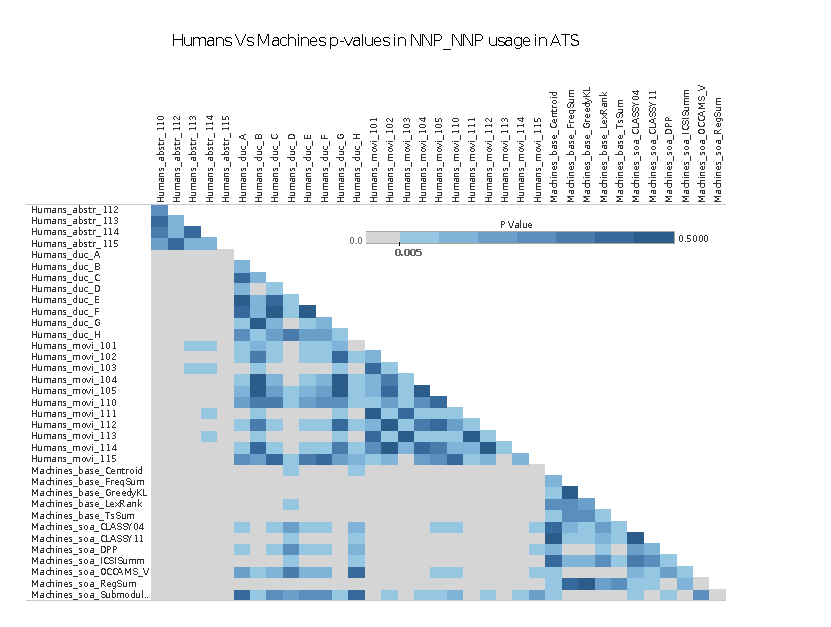
\includegraphics[
%trim={8 17cm 8cm 10},clip,
width=8.7cm,height=7.5cm]{Figure_7}
\end{figure}
%trim={<left> <lower> <right> <upper>}

As it is known in Information Theory, the information amount of a word is directly related with its frequency of occurrence within a context. Taking the frequency of the proper noun bigrams generated by humans as a reference (\xref{fig:NNP_NNP}), it was barely surpassed by state-of-the-art machines (except by \texttt{Machines\_}\ubrk\texttt{soa\_Submodular}) and completely left behind by baseline ones (except probably by \texttt{Machines\_base\_Centroid}). 

In general, machines probably do not take into consideration the expected
information amount of the lexical items contained in the summaries they
produce. In the case of the features analyzed at this point, it seems that
machines simply try to keep a set of predefined features of source documents as
frequent as possible in the resulting summaries, rather than keeping them
informative. We think that this bias could affect the informativeness of the
summaries considerably. This lack of informativeness could also be a potential
factor affecting the quality of machine summaries so as to be easily
identifiable by humans in Turing-like evaluation
tests~\cite{lowe2017towards,molina2013turing,pitler2010automatic}. 

It was interesting that another feature that was pertinent to distinguish human
from machine summaries was the moderate amount of neutral sentiments used by
humans to express the information in the source documents (at least from the
point of view of the sentiment polarities the coreNLP classifier assigned).
This behavior can also be observed in the statistics shown
by~\cite{socher2013recursive} for the Stanford Sentiment Treebank, which is a
human-annotated sentiment classification dataset. The boxplots showed that this
behavior was imitated by state-of-the-art summarizers; however,
\texttt{Machines\_soa\_RegSum} was a notable exception
(\xref{fig:tok_sentim_2}). This summarizer was shown to be statistically
distinct from humans and state-of-the-art summarizers in that it presented high
variability and frequent use of neutral tokens. 

\begin{figure*}%8
\caption{\xlabel{Figure_8}Boxplot of (a) the neutral sentiment by token feature (tok\_sentim\_2) and of (b) positive sentiment sentences feature (sent\_sentim\_3) through all summaries. Horizontal axis indicates the human/machine summary. Vertical axis indicates the frequency of occurrence of the feature.}
\subfigure[]{\xlabel{fig:tok_sentim_2}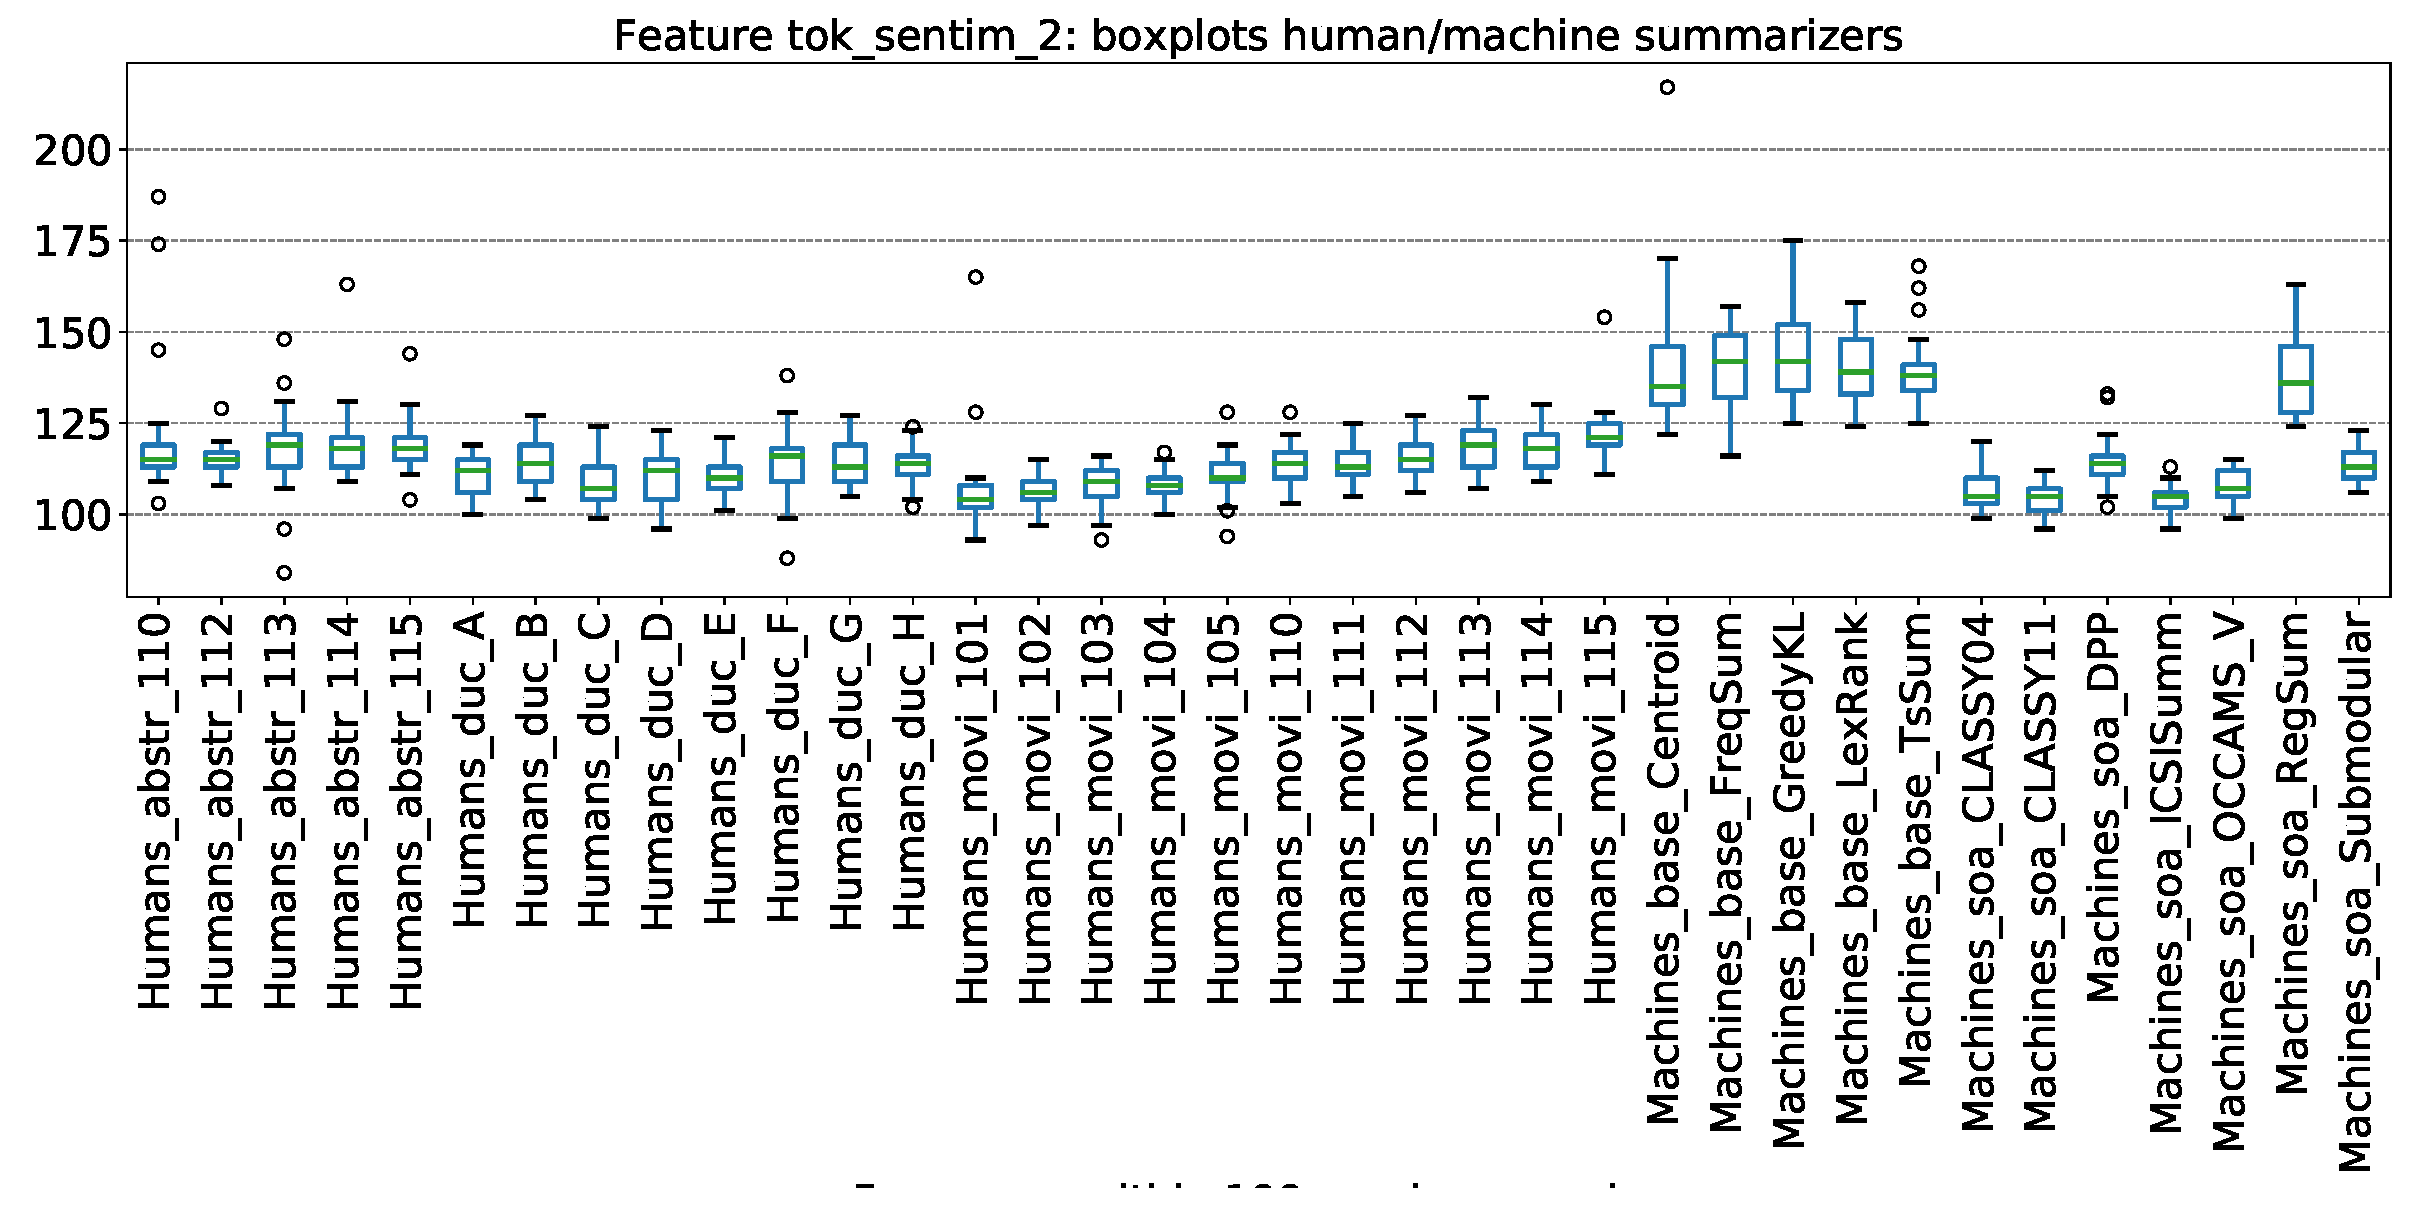
\includegraphics[scale=0.25]{Figure_8a}}
\subfigure[]{\xlabel{fig:sent_sentim_3}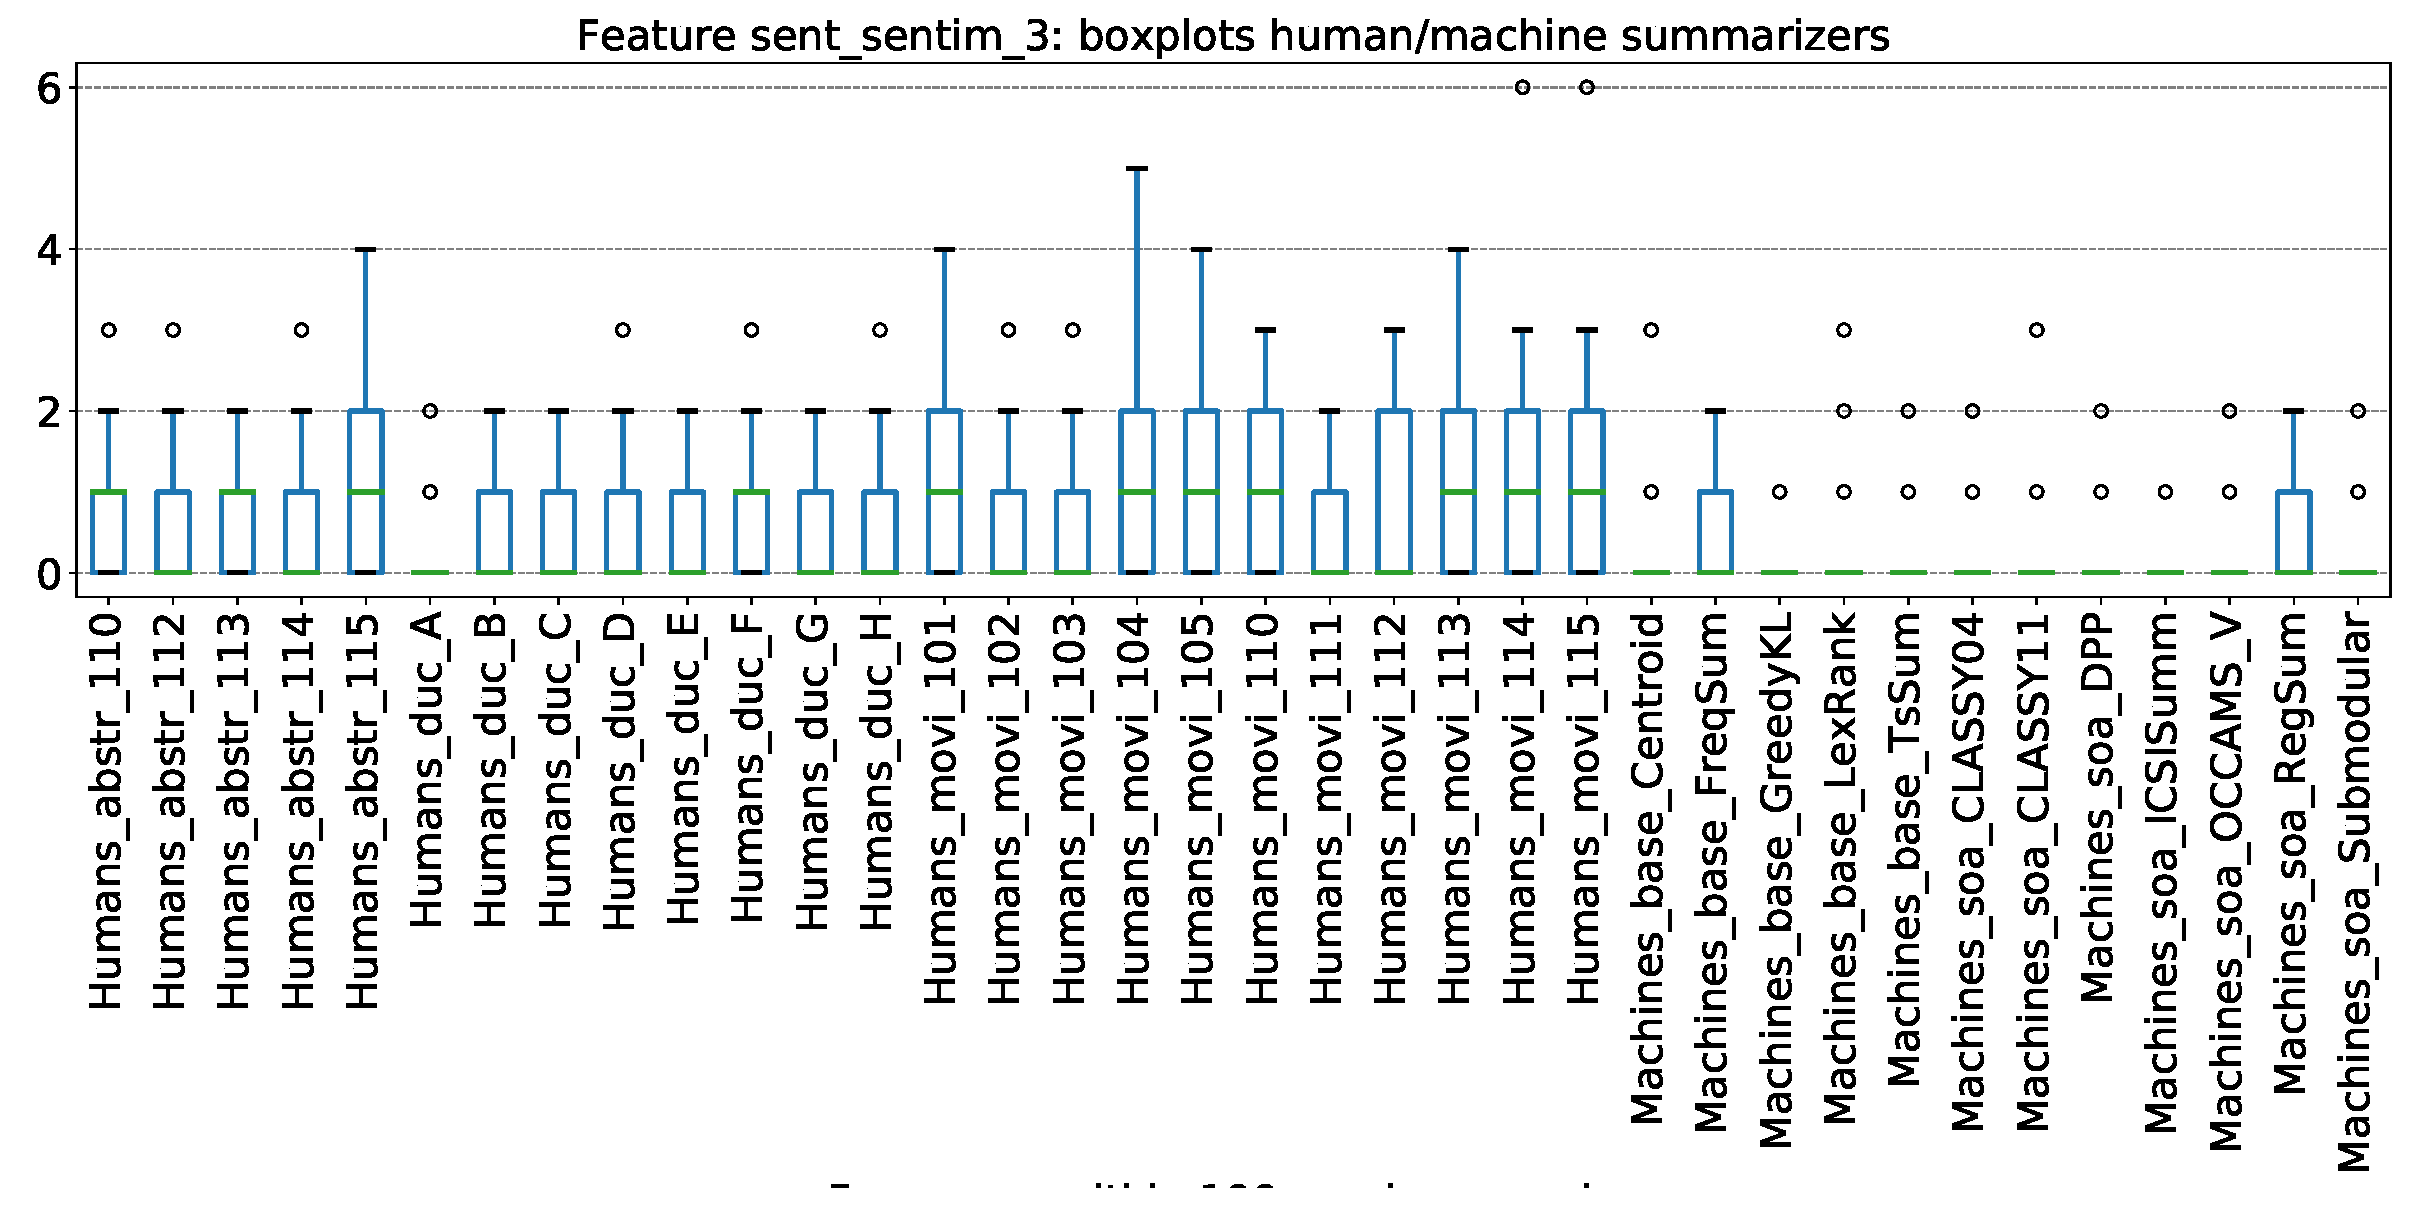
\includegraphics[scale=0.25]{Figure_8b}}
\end{figure*}

Sentiment polarity at the sentence level, gave us complementary information about what the sentiment tagger did at token level. We observed a possible consequence of high use of neutral words by machines. While machines tend to \textit{neutralize} sentiments (\xref{fig:tok_sentim_2}), humans tend always to express some emotional signal. Observe the scarcity of positive sentences selected by machines in the right hand side of \xref{fig:sent_sentim_3}. Notice that this difference is relatively distinguishable by contrasting neutral sentiment tokens and positive sentiment sentences (\texttt{sent\_sentim\_3}). Similar patterns can be observed for the negative sentiment (for tokens and sentences), although, in those cases, the tendency is much less noticeable. Notably, a baseline summarizer and the \texttt{Machines\_soa\_RegSum} were the most similar to humans in the use of this feature. Taking into account previously observed behavior of \texttt{Machines\_soa\_RegSum}, if we exclude it from the group of state-of-the-art summarizers, the neutral sentiment of tokens (\xref{fig:tok_sentim_2}) in fact resulted in a statistically pertinent feature to distinguish baseline summarizers from humans and state-of-the-art summarizers.

For simplicity, in \xref{fig:sent_sentim_3_heatmap} we show the $p$-values between the distribution of sentences with positive sentiment present in human and machine-made summaries of the development data. Notice that, in most cases, the $H_0$ hypothesis suggested by boxplots for this feature resulted worth supporting. That is, with high probability, machines have not the ability of expressing positive sentiments when drawing sentences from source documents to build summaries.

\begin{figure}%9
\caption{Mann--Whitney U test for \texttt{sent\_sentim\_3} bigrams usage in human-made and machine-made summaries\xlabel{fig:sent_sentim_3_heatmap}}
\includegraphics[width=8.7cm,height=7.5cm]{Figure_9}
\end{figure}


The analysis of features of the manual summaries from news articles performed
in~\cite{hong2014improving} showed that entities such as persons, organizations
and locations tend to appear in human summaries whereas time and dates do not.
We confirmed the behavior for \texttt{DATE} and observed that, contrary to
human behavior, machines tend to select sentences including these entities.
This pattern for \texttt{DATE} was observed less markedly for entity mentions like persons,
organizations and locations: humans tend to include these entities moderately in
summaries, but machines tend to include them frequently. Concerning the patterns
observed for sentiment polarity (in~\cite{hong2014improving} this kind of feature
indicates subjectivity), we confirmed the fact that strong sentiments (very positive or very negative) do not tend to appear in the summaries studied here. We also observed that machine-made summaries tend to lack positive and negative sentiments, and neutral sentiment tokens are systematically present in baseline machine summaries.

\begin{figure}%10
\caption{Mann--Whitney U test for \texttt{named\_entities} mentions in human-made and machine-made summaries\xlabel{fig:named_entities_heatmap}}
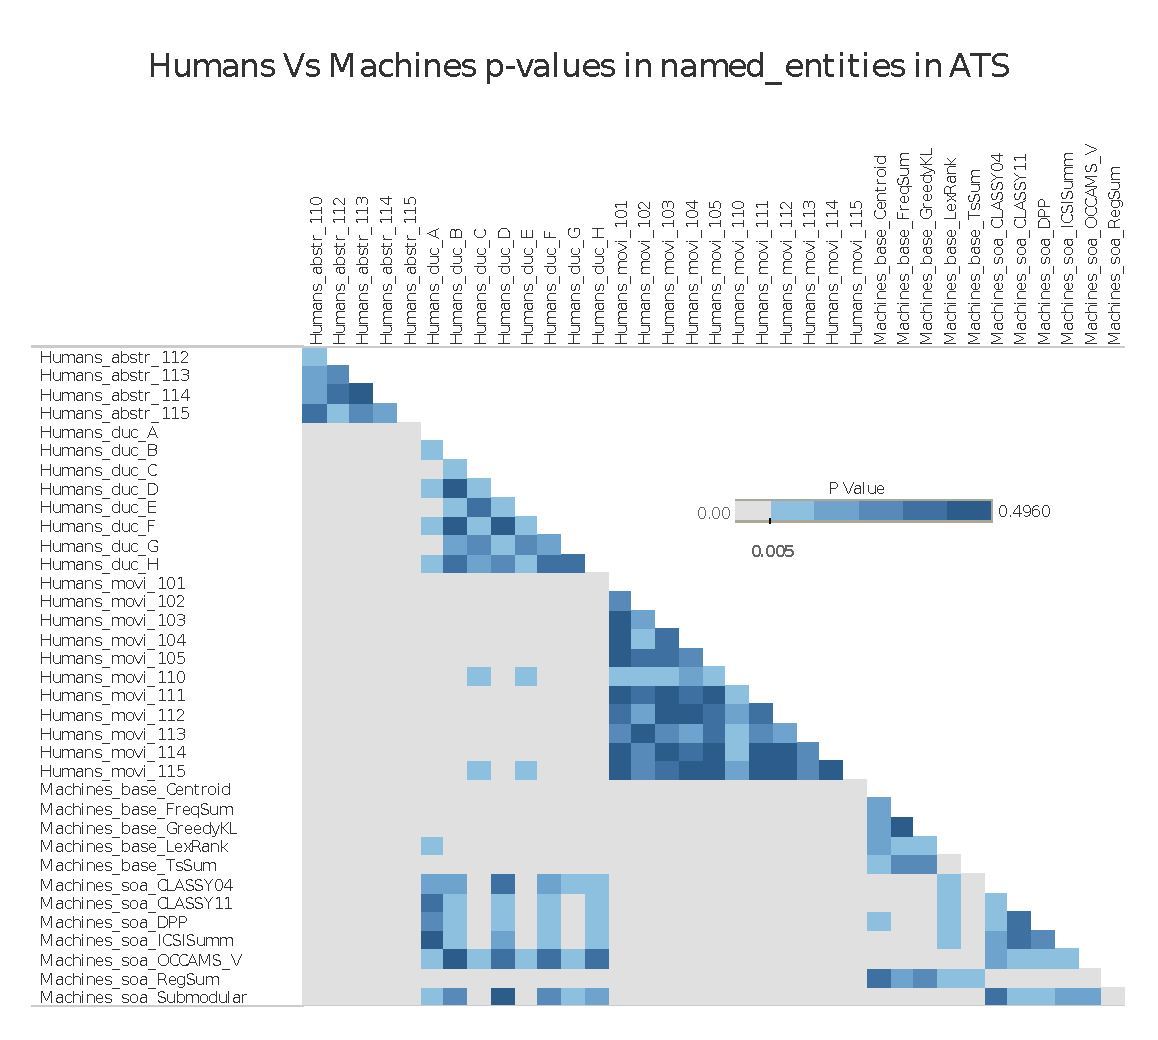
\includegraphics[width=8.7cm,height=7.5cm]{Figure_10}
\end{figure}

Not all the features suggested as pertinent by the Feature Spectrum analysis were deemed useful to distinguish between humans and machines, as given by the corresponding hypothesis test results. For instance, \texttt{named\_entities} is an interesting case because most ATS methods take considerable effort to keep them from source documents to their summaries. The corresponding hypothesis test showed that this feature in fact is not regularly distributed through the different types of human-made summaries we analyzed in this paper (see \xref{fig:named_entities_heatmap}), except for some human summaries of the DUC dataset. To build these latter summaries, state-of-the-art summarizers used the same kind of source documents, which may explain statistical dependencies with respect to DUC human-made summaries. As shown in the heatmap, statistical independencies suggest that probably named entities are not good features to judge either $H_0$ or $H_1$ as these features show statistical properties that rather favor the distinction of different kinds of source documents. Overall, named entities do not seem to be ideal if we would want to use them to emulate human behavior when doing summaries. Notice that these results hold uniquely for the datasets we studied and for the criteria we assumed in this work, which do not attempt to be valid for all possible summaries.

\begin{figure}%11
\caption{Mann--Whitney U test for \texttt{TotalRST} usage in human-made and machine-made summaries\xlabel{fig:rst_heatmap}}
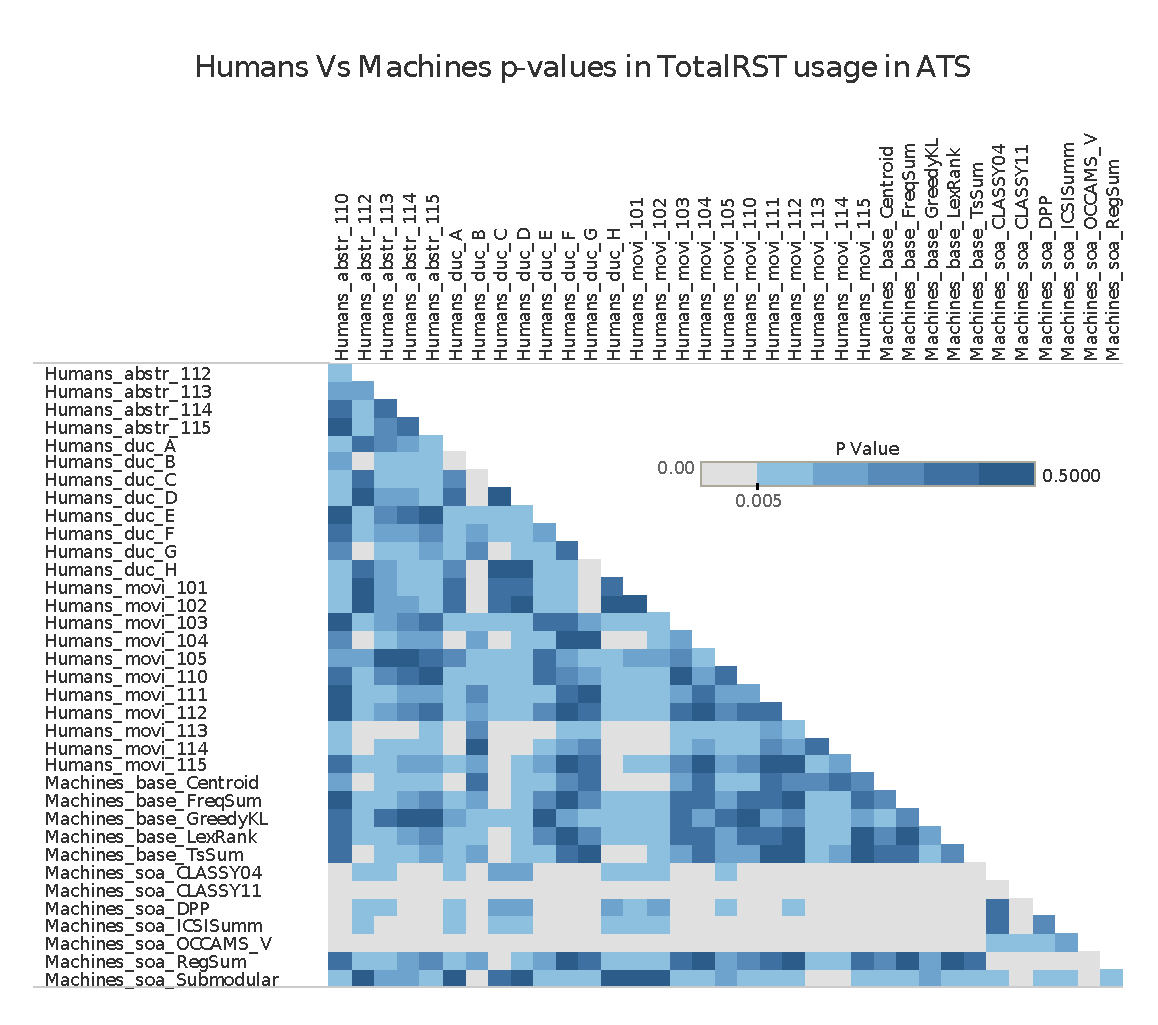
\includegraphics[width=8.7cm,height=7.5cm]{Figure_11}
\end{figure}

Another interesting case suggested as pertinent by the Feature Spectrum analysis, that was not analyzed via boxplots, was \texttt{TotalRST} (frequency of all categories of Rhetorical-Structure-Theoretical EDUs. See \xref{fig:rst_heatmap}). This was interesting for us because in fitting data it showed to have a negative level of usage with respect to humans. Also it was interesting because this kind of feature is used in few ATS methods, although our results showed it as a good indicator of that the alternative hypothesis $H_1$ (statistical dependency) cannot be safely accepted. Interestingly, it occurred for most state-of-the-art summarizers. Contrarily, $H_1$ is worthy of acceptance for most baseline summarizers with respect to the \texttt{TotalRST} feature.

\section{Conclusions}
\xlabel{sec05:conclusions}

Results obtained by means of comparing boxplots showed an imbalanced use of some features by state-of-the-art and baseline summarizers compared to humans. Date mentions are almost absent in human summaries, but they are present in machine summaries. In addition, bigrams of proper nouns and neutral sentiments per word are used moderately by humans, but they appear frequently in machine-made summaries. Also, positive sentiment sentences tend to be present in human-made summaries, but are almost completely absent in machine-made summaries. 

Regarding PoS tags, we found that noun forms were used excessively by machines. This prevented them from taking into account other structural features that may contribute to the informativeness of the summaries. For instance, the Feature Spectrum showed negative usage level of RST features, which in turn is closely related with the lack of coordinating conjunctions (\texttt{CC}), at the discourse level. This latter syntactic feature plays an important role in information compression (e.g.~by including information from other sentences in the form of arguments) as the speakers use it to elaborate, to support or to emphasize their ideas~\cite{asher2005subordinating}. Therefore, these are abilities that seem to be absent in machines studied in this work. We consider this reasoning relevant to say that relevance is not only encoded in lexical items of text, but also in the structure of language.

Lacks and excesses found in fitting data were supported via hypothesis tests, on development data with $95\%$ of confidence. This was specially useful when we analyzed named entities, which resulted difficult to assess only by means of the Feature Spectrum and the boxplot analyses. In this case, hypothesis tests provided additional accuracy, which helped to judge the original hypotheses suggested by fitting data analysis. Named entities resulted not useful to compare our groups of summaries. This led us to conclude that focusing summaries on this feature is not the best fit. Overall, moderation and low variability is an important trait humans keep for most of the noun form features they use when summarizing.

The area of Artificial Intelligence could benefit from our findings as they describe lacks and excesses of ATS approaches. On the one hand, the Feature Spectrum combined with boxplots were useful tools for general and fine-grained analysis of the mentioned lacks and excesses determined by taking human-made summaries as reference behaviors. On the other hand, hypothesis testing on development data helped to support the hypotheses suggested by fitting data analysis. We offer insight on how, consciously or unconsciously, humans use well known language features via their intellect (either to generate or to evaluate summaries). Thus, ATS methods (also probably language generation approaches) and evaluation techniques can be revisited considering features beyond lexical overlapping, which we conclude that is an incomplete approach in the sense of imitating human behavior. 

\ackheads 
With thank to: \grantsponsor{CONACyT\gcny*{Mexico}}[http://dx.doi.org/10.13039/501100003141] (Grant \grantnumber{1}{386128}), \grantsponsor{Laboratorio Universitario de
c\'omputo de alto rendimiento (IIMAS--UNAM)\gcny*{Mexico}} and \grantsponsor{The Computational Genomics
Research Program (PGC/CCG--UNAM)\gcny*{Mexico}} for their valuable support. Arturo Curiel
(CVU: \grantnumber{3}{268370}) is supported by the \grantsponsor{C\'atedras CONACYT program\gcny*{Mexico}}[http://dx.doi.org/10.13039/501100003141] and the project
%\QUERY[7]
entitled \textit{``Infraestructura para agilizar el desarrollo de sistemas
centrados en el usuario''} (Ref. 3053). And thank you very much to
\textit{Juana Arroyo \'{A}ngel} for your proofread. 






%\QUERY[8]
\appendix{}
\section[cpt,idstr=appS,pfx=Appendix\space]{Supplementary material}

\xlabel{sec:appendix}

%\stext[cpt]
Supplementary material related to this article can be found online at \myehost{https://github.com/iarroyof/summ_features/blob/master/KNOSYS-D-18-02363R1_supplementary.pdf}.

\section[ext,idstr=appS,num=A,pfx=Appendix\space]{Supplementary material}

\stext[ext]

\begin{mmc}[type=e-component,
  label={MMC S1},
  id={mmc1},extn={zip}]
   \linkloc{mmc1}
\end{mmc}




\endextsection

\back{}

\nocite{*}

\bibliographystyle{stm-xml-sort-num-fnm-abre}

\bibliography{\jobname}


\begin{bibwrite}{\jobname.bib}
%\QUERY[9]
@article{radev2002introduction,
 serialno={1},
 author={Radev, Dragomir R. and Hovy, Eduard and McKeown, Kathleen},
 year={2002},
title={Introduction to the special issue on summarization},
 journal={Comput. Linguist.},
 volume={28},
 number={4},
  pages={399--408},
 orgname = {MIT Press},
 
}


@article{gambhir2017recent,
 serialno={2},
 author={Gambhir, Mahak and Gupta, Vishal},
 year={2017},
title={Recent automatic text summarization techniques: a survey},
 journal={\rvtAIR},
 volume={47},
 number={1},
  pages={1--66},
 orgname = {Springer},
}


@article{barry_user-defined_1994,
 serialno={3},
 author={Barry, Carol L.},
 year={1994},
title={User-defined relevance criteria: \?{A}n exploratory study},
 journal={J. Am. Soc. Inf. Sci.},
 volume={45},
 number={3},
  pages={149--159},
}


@article{barry_users_1998,
 serialno={4},
 author={Barry, Carol L. and Schamber, Linda},
 year={1998},
title={Users' criteria for relevance evaluation: \?{A} cross-situational
  comparison},
 journal={\rvtInfPro},
 volume={34},
 number={2},
  pages={219--236},
}


@article{taylor_user_2012,
 serialno={5},
 author={Taylor, Arthur},
 year={2012},
title={User relevance criteria choices and the information search process},
 journal={\rvtInfPro},
 volume={48},
 number={1},
  pages={136--153},
 keywords={Information retrieval, Information search process, Relevance,
  Relevance criteria},
}


@article{nandhini_improving_2013,
 serialno={6},
 author={Nandhini, K. and Balasundaram, S. R.},
 year={2013},
title={Improving readability through extractive summarization for learners
  with reading difficulties},
 journal={Egypt. Inform. J.},
 volume={14},
 number={3},
  pages={195--204},
 keywords={Assistive reading, Extractive summarization, Machine learning, Naive
  Bayes classifier, Text summarization},
}


@inbook{conroy2008mind,
 serialno={7},
 author={Conroy, John M. and Dang, Hoa Trang},
 year={2008},
title={Mind the gap: \?{D}angers of divorcing evaluations of summary content from
  linguistic quality},
 booktitle={Proceedings of the 22nd International Conference on Computational
  Linguistics-Volume 1},
  pages={145--152},
 organization={Association for Computational Linguistics},
}


@inbook{lin:2004rpa,
 serialno={8},
 author={Lin, Chin-Yew},
 year={2004},
title={{ROUGE}: \?{A} Package for Automatic Evaluation of Summaries},
 booktitle={Workshop Text Summarization Branches Out (ACL'04)},
  pages={74--81},
 orgname = {ACL},
 city = {Barcelona, Spain},
 editor={Marie-Francine Moens and Stan Szpakowicz},
}


@inbook{galanis2012extractive,
 serialno={9},
 author={Galanis, Dimitrios and Lampouras, Gerasimos and Androutsopoulos, Ion},
 year={2012},
title={Extractive Multi-Document Summarization with Integer Linear Programming
  and Support Vector Regression.},
 booktitle={COLING},
  pages={911--926},
}


@inbook{kdir16,
 serialno={10},
 author={Ignacio Arroyo-Fern\'andez and Juan-Manuel Torres-Moreno and Gerardo
  Sierra and Luis Adrin Cabrera-Diego},
 year={2016},
title={Automatic Text Summarization by Non-topic Relevance Estimation},
 booktitle={Proceedings of the 8th International Joint Conference on Knowledge
  Discovery, Knowledge Engineering and Knowledge Management - Volume 1: KDIR,
  (IC3K 2016)},
  pages={89--100},
 orgname = {INSTICC, ScitePress},
}


@article{BHARGAVA2016404,
 serialno={11},
 author={Rupal Bhargava and Yashvardhan Sharma and Gargi Sharma},
 year={2016},
title={{ATSSI}: \?{A}bstractive Text Summarization Using Sentiment Infusion},
 journal={\rvtPComS},
 volume={89},
  pages={404--411},
 keywords={Abstractive Summarization, Condensed Text, Data Redundancy,
  Sentiment Analysis, Summary, Text Summarization},
 note={Twelfth International Conference on Communication Networks, ICCN 2016,
  August 19 21, 2016, Bangalore, India Twelfth International Conference on
  Data Mining and Warehousing, ICDMW 2016, August 19-21, 2016, Bangalore, India
  Twelfth International Conference on Image and Signal Processing, ICISP 2016,
  August 19-21, 2016, Bangalore, India},
}


@inbook{hong2014improving,
 serialno={12},
 author={Hong, Kai and Nenkova, Ani},
 year={2014},
title={Improving the estimation of word importance for news multi-document
  summarization},
 booktitle={Proceedings of the 14th Conference of the European Chapter of the
  Association for Computational Linguistics},
  pages={712--721},
}


@incollection{SMALHEISER2017157,
 serialno={13},
 author={Neil R. Smalheiser},
 year={2017},
title={Chapter 12 - Nonparametric Tests},
 booktitle={Data Literacy},
  pages={157--167},
 orgname = {Academic Press},
 editor={Neil R. Smalheiser},
}


@inbook{hong2014repository,
 serialno={14},
 author={Hong, Kai and Conroy, John M and Favre, Benoit and Kulesza, Alex and
  Lin, Hui and Nenkova, Ani},
 year={2014},
title={A Repository of State of the Art and Competitive Baseline Summaries for
  Generic News Summarization},
 booktitle={LREC},
  pages={1608--1616},
}


@article{du2009confidence,
 serialno={15},
 author={du Prel, Jean-Baptist and Hommel, Gerhard and R{\"o}hrig, Bernd and
  Blettner, Maria},
 year={2009},
title={Confidence interval or p-value?: part 4 of a series on evaluation of
  scientific publications},
 journal={Deutsch. {\"A}rzteblatt Int.},
 volume={106},
 number={19},
  pages={335},
 orgname = {Deutscher Arzte-Verlag GmbH},
}


@article{harris1957co,
 serialno={16},
 author={Harris, Zellig S.},
 year={1957},
title={Co-occurrence and transformation in linguistic structure},
 journal={Language},
 volume={33},
 number={3},
  pages={283--340},
 orgname = {JSTOR},
}


@book{Harris1991information,
 serialno={17},
 author={Harris, Zellig Sabbettai},
 year={1991},
booktitle={Theory of Language and Information: {A} Mathematical Approach},
 orgname = {Oxford University Press UK},
}


@article{jones1999automatic,
 serialno={18},
 author={Jones, Karen Sp\"arck},
 year={1999},
title={Automatic summarizing: factors and directions},
 journal={Advances in automatic text summarization},
  pages={1--12},
 orgname = {MIT Press},
 city={Cambridge, MA},
}


@inbook{dabholkar2016automatic,
 serialno={19},
 author={Dabholkar, Salil and Patadia, Yuvraj and Dsilva, Prajyoti},
 year={2016},
title={Automatic Document Summarization using Sentiment Analysis},
 booktitle={Proceedings of the International Conference on Informatics and
  Analytics},
  pages={49},
 organization={ACM},
}


@inbook{yadav2016text,
 serialno={20},
 author={Yadav, Nidhika and Chatterjee, Niladri},
 year={2016},
title={Text Summarization Using Sentiment Analysis for {DUC} Data},
 booktitle={Information Technology (ICIT), 2016 International Conference on},
  pages={229--234},
 organization={IEEE},
}


@article{grosz1986attention,
 serialno={21},
 author={Grosz, Barbara J. and Sidner, Candace L.},
 year={1986},
title={Attention, intentions, and the structure of discourse},
 journal={Comput. Linguist.},
 volume={12},
 number={3},
  pages={175--204},
 orgname = {MIT Press},
 aetag={\xvfill\xeject},
}


@article{mann1988rhetorical,
 serialno={22},
 author={Mann, William C. and Thompson, Sandra A.},
 year={1988},
title={Rhetorical structure theory: \?{T}oward a functional theory of text
  organization},
 journal={Text-Interdiscip. J. Study Discourse},
 volume={8},
 number={3},
  pages={243--281},
 orgname = {Walter de Gruyter, Berlin/New York},
}


@inbook{manning2014corenlp,
 serialno={23},
 author={Manning, Christopher D. and Surdeanu, Mihai and Bauer, John and  Finkel, Jenny and Bethard, Steven J. and McClosky, David},
 year={2014},
title={The \?{Stanford} \?{CoreNLP} Natural Language Processing Toolkit},
 booktitle={Association for Computational Linguistics (ACL) System  Demonstrations},
  pages={55--60},
}


@inbook{socher2013recursive,
 serialno={24},
 author={Socher, Richard and Perelygin, Alex and Wu, Jean Y and Chuang, Jason
  and Manning, Christopher D and Ng, Andrew Y and Potts, Christopher},
 year={2013},
title={Recursive deep models for semantic compositionality over a sentiment
  treebank},
 booktitle={Conference on Empirical Methods in Natural Language Processing
  (EMNLP)},
  pages={1631--1642},
}


@inbook{feng2014linear,
 serialno={25},
 author={Feng, Vanessa Wei and Hirst, Graeme},
 year={2014},
title={A linear-time bottom-up discourse parser with constraints and
  post-editing},
 booktitle={Proceedings of the 52nd Annual Meeting of the Association for
  Computational Linguistics (Volume 1: Long Papers), Vol. 1},
  pages={511--521},
}


@article{deardorff2016tableau,
 serialno={26},
 author={Deardorff, Ariel},
 year={2016},
title={Tableau (version. 9.1)},
 journal={J. Med. Libr. Assoc.},
 volume={104},
 number={2},
  pages={182--183},
}


@inbook{mckinney-proc-scipy-2010,
 serialno={27},
 author={Wes McKinney},
 year={2010},
title={Data Structures for Statistical Computing in Python},
 booktitle={Proceedings of the 9th Python in Science Conference},
  pages={51--56},
 editor={St\'efan van der Walt and Jarrod Millman},
}


@article{Hunter:2007,
 serialno={28},
 author={Hunter, J. D.},
 year={2007},
title={Matplotlib: \?{A} 2D graphics environment},
 journal={Comput. Sci. Eng.},
 volume={9},
 number={3},
  pages={90--95},
 orgname = {IEEE COMPUTER SOC},
}


@book{fano1949transmission,
 serialno={29},
 author={Fano, Robert M.},
 year={1949},
booktitle={The Transmission of Information},
 orgname = {Massachusetts Institute of Technology, Research Laboratory of
  Electronics Cambridge, Mass, USA},
}


@article{huffman1952method,
 serialno={30},
 author={Huffman, David A.},
 year={1952},
title={A method for the construction of minimum-redundancy codes},
 journal={Proc. IRE},
 volume={40},
 number={9},
  pages={1098--1101},
 orgname = {IEEE},
}


@inbook{herbelot2013measuring,
 serialno={31},
 author={Herbelot, Aur{\'e}lie and Ganesalingam, Mohan},
 year={2013},
title={Measuring semantic content in distributional vectors},
 booktitle={Proceedings of the 51st Annual Meeting of the Association for
  Computational Linguistics (Volume 2: Short Papers), Vol. 2},
  pages={440--445},
}


@inbook{shah2002study,
 serialno={32},
 author={Shah, Chirag and Bhattacharyya, Pushpak},
 year={2002},
title={A study for evaluating the importance of various parts of speech ({POS})
  for information retrieval ({IR})},
 booktitle={Proc. International Conference on Universal Knowledge and
  Languages, ICUKL},
}


@inbook{mishra2011predicting,
 serialno={33},
 author={Mishra, Taniya and Bangalore, Srinivas},
 year={2011},
title={Predicting relative prominence in noun-noun compounds},
 booktitle={Proceedings of the 49th Annual Meeting of the Association for
  Computational Linguistics: Human Language Technologies: Short Papers-Volume
  2},
  pages={609--613},
 organization={Association for Computational Linguistics},
}


@others{lowe2017towards,
 serialno={34},
 author={Lowe, Ryan and Noseworthy, Michael and Serban, Iulian V and
  Angelard-Gontier, Nicolas and Bengio, Yoshua and Pineau, Joelle},
commn={Towards an automatic turing test: Learning to evaluate dialogue
responses, arXiv preprint \myehost{arXiv:1708.07149}, 2017},
}


@inbook{molina2013turing,
 serialno={35},
 author={Molina, Alejandro and SanJuan, Eric and Torres-Moreno, Juan-Manuel},
 year={2013},
title={A turing test to evaluate a complex summarization task},
 booktitle={International Conference of the Cross-Language Evaluation Forum for
  European Languages},
  pages={75--80},
 organization={Springer},
}


@inbook{pitler2010automatic,
 serialno={36},
 author={Pitler, Emily and Louis, Annie and Nenkova, Ani},
 year={2010},
title={Automatic evaluation of linguistic quality in multi-document
  summarization},
 booktitle={Proceedings of the 48th Annual Meeting of the Association for
  Computational Linguistics},
  pages={544--554},
 organization={Association for Computational Linguistics},
}


@article{asher2005subordinating,
 serialno={37},
 author={Asher, Nicholas and Vieu, Laure},
 year={2005},
title={Subordinating and coordinating discourse relations},
 journal={\rvtLingua},
 volume={115},
 number={4},
  pages={591--610},
 orgname = {Elsevier},
}

\end{bibwrite}




\newbox\uncitedrefsbox
\setbox\uncitedrefsbox=\vbox{\xref[nosort]{TeXFolio:fig6,TeXFolio:fig8}}

\end{document}
